\scanpage{19}
% archive sheet number: 18
\uline{Proposition}\qquad Soient $\Gamma,\Gamma'$ deux J.polygônes \unsure{sur|du} plan $E$, tels que $\Gamma\cap\Gamma'=I$ soit un arc polygonal non réduit \unsure{à|:} un point. Alors on est dans l'un des deux cas suivants (s'excluant mutuellement)

\[
\begin{aligned}
 &\mathrm{a)}\quad \Gamma-I\subset\mathrm{Ext}(\Gamma'),\quad
 \Gamma'-I\subset\mathrm{Ext}(\Gamma)\\
 &(\Longleftrightarrow\quad \mathrm{Int}\,\Gamma'\subset\mathrm{Ext}\,\Gamma,\quad
 \mathrm{Int}\,\Gamma\subset\mathrm{Ext}\,\Gamma')
\end{aligned}
\]
\[
\begin{aligned}
 &\mathrm{b)}\quad\Gamma-I\subset\mathrm{Ext}\,\Gamma',\quad
 \Gamma'-I\subset\mathrm{Int}\,\Gamma\quad \text{(ou inversement)}\\
 &(\Longleftrightarrow\quad \mathrm{Int}\,\Gamma'\subset\mathrm{Int}\,\Gamma,\quad
 \mathrm{Ext}(\Gamma)\subset\mathrm{Ext}\,\Gamma'\quad \text{(ou inv.)})
\end{aligned}
\]

\deleted{\unsure{a)|$\alpha$)} Dans le cas a),}
Soit $\Gamma''=(\Gamma\cup\Gamma')-(I\unsure{\setminus|-}\partial I)
=\overline{\Gamma-I}\cup\overline{\Gamma'-I}$, qui est un polygône.
C'est un J-polygône, et \unsure{on a} :

\[
\begin{aligned}
 \text{\uline{Cas a)}}\quad \mathrm{Int}\,\Gamma''&=\mathrm{Int}\,\Gamma\cup\mathrm{Int}\,\Gamma'\cup(I-\partial I)\\
 \mathrm{Ext}\,\Gamma''&=\mathrm{Ext}\,\Gamma\cap\mathrm{Ext}\,\Gamma'
\end{aligned}
\]
% The circled item in the second line is carried up to the gap after en.
\noindent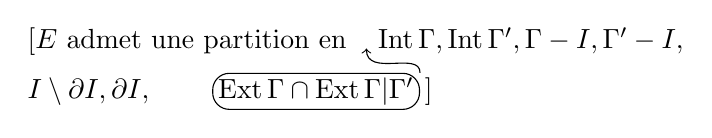
\begin{tikzpicture}[baseline=(lead.base)]
\node[anchor=base west,inner sep=0pt] (lead) at (0,0) {[$E$ admet une partition en};
\node[anchor=base west,inner xsep=2pt,inner ysep=1.5pt,draw,rounded corners=6pt]
 (moved) at (2.35cm,-1.8em)
 {\inserted{$\mathrm{Ext}\,\Gamma\cap\mathrm{Ext}\,\unsure{\Gamma|\Gamma'}$}};
\node[anchor=base west,inner sep=0pt] at ([xshift=1.1em]lead.base east)
 {$\mathrm{Int}\,\Gamma,\mathrm{Int}\,\Gamma',\Gamma-I,\Gamma'-I,$};
\node[anchor=base west,inner sep=0pt] at (0,-1.8em) {$I\setminus\partial I,\partial I,$};
\node[anchor=base west,inner sep=0pt] at ([xshift=.15em]moved.base east) {]};
\draw[->] (moved.north east) .. controls +(0,.8em) and +(0,-1.05em)
 .. ([xshift=.7em]lead.base east);
\end{tikzpicture}

\[
\begin{aligned}
 \text{\uline{Cas b)}}\quad \mathrm{Int}\,\Gamma''&=
 \mbox{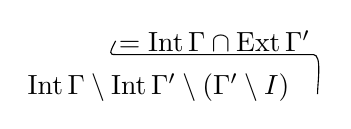
\begin{tikzpicture}[baseline=(mainterm.base)]
 \node[anchor=base west,inner sep=0pt] (mainterm) at (0,0)
 {$\mathrm{Int}\,\Gamma\setminus\mathrm{Int}\,\Gamma'\setminus(\Gamma'\setminus I)$};
 \node[anchor=base east,inner sep=1pt] (addition)
 at ([xshift=.85em,yshift=1.55em]mainterm.base east)
 {$\inserted{=\mathrm{Int}\,\Gamma\cap\mathrm{Ext}\,\Gamma'}$};
 \draw (addition.west) .. controls +(-.23em,-.45em) and +(-.24em,0) .. (addition.south west)
 -- (addition.south east) .. controls +(.32em,0) and +(0,.42em)
 .. ([xshift=1em]mainterm.base east);
 \end{tikzpicture}}\\
 \mathrm{Ext}\,\Gamma''&=\mathrm{Ext}\,\Gamma\cup\mathrm{Int}\,\Gamma'\cup(I\setminus\partial I)
\end{aligned}
\]
[$E$ admet une partition en \inserted{$\mathrm{Ext}\,\Gamma$}
$\mathrm{Int}\,\Gamma\cap\mathrm{Ext}\,\Gamma',\mathrm{Int}\,\Gamma',$
\deleted{$\mathrm{Ext}\,\Gamma$}
$\Gamma-I,\Gamma'-I,I-\partial I,\partial I$]
